%!TEX options=--shell-escape
\documentclass[tikz]{standalone}
\usepackage[T1]{fontenc}
\usepackage[utf8]{inputenc}
\usepackage{xcolor}
\usepackage{amsmath}
\usepackage{amssymb}
\usepackage{hyperref}
\usepackage{accsupp}    
\usepackage{graphicx}
\usepackage{mathtools}
\usepackage{pagecolor}
\usepackage{amsmath} % for \dfrac
\usepackage{tikz}
\tikzset{>=latex} % for LaTeX arrow head
\usepackage{pgfplots} 
\usepackage[edges]{forest}
\usetikzlibrary{patterns, backgrounds, arrows.meta}
\setlength{\parindent}{0cm}
\setlength{\parskip}{1em}
\usepackage{braket}

\usetikzlibrary{patterns}

% Figure 4.3 https://arxiv.org/pdf/1709.02318.pdf 

\begin{document}
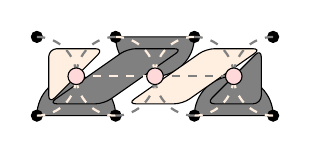
\begin{tikzpicture}[]

 \foreach \x in {0}{
    \draw[black, fill=gray](\x + 1,1) arc (0:180:-0.5) -- cycle;
    \draw[black, fill=gray](\x,0) arc (180:0:0.5) -- cycle;
    } 
    \draw[black, fill=gray](2,0) arc (180:0:0.5) -- cycle;

   \foreach \x in {0}{
       \fill[draw=black, fill=gray, rounded corners=3pt] (\x + 0.15, 0.15) -- (\x + 1.15, 0.85) -- (\x+1.85, 0.85) -- (\x+0.85, 0.15)  -- cycle;
        }

    \foreach \x in {1}{
   \fill[draw=black, fill=yellow!40!red!10, rounded corners=3pt] (\x + 0.15, 0.15) -- (\x + 1.15, 0.85) -- (\x+1.85, 0.85) -- (\x+0.85, 0.15)  -- cycle;
    }


% End Cap
    \fill[draw=black, fill=yellow!40!red!10, rounded corners=3pt] (0.15, 0.15) -- (0.15, 0.85) -- (0.85, 0.85) -- cycle ;

\fill[draw=black, fill=gray, rounded corners=3pt] (2.85, 0.85) -- (2.15, 0.15) -- (2.85, 0.15) -- cycle ;

    \foreach \x in {0, 1}{
           \filldraw[draw=black, fill=black] (2*\x, 0) circle[radius=2pt] node[font=\tiny] {};
           \filldraw[draw=black, fill=black] (2*\x + 1, 0) circle[radius=2pt] node[font=\tiny] {};
           \filldraw[draw=black, fill=black] (2*\x, 1) circle[radius=2pt] node[font=\tiny] {};
           \filldraw[draw=black, fill=black] (2*\x + 1, 1) circle[radius=2pt] node[font=\tiny] {};
    }

    \draw[thick, dashed, gray] (1.5, 0.5) to (2.5, 0.5);
    \draw[thick, dashed, yellow!40!red!10] (0.5, 0.5) to (1.5, 0.5);

    \foreach \x in {1}{
        \draw[thick, dashed, gray] (\x, 0) to [bend right=45](\x+0.5, 0.5);
        \draw[thick, dashed, gray] (\x + 1, 0) to [bend left=45](\x+0.5, 0.5);

        \draw[thick, dashed, yellow!40!red!10] (\x, 1) to [bend left=45](\x+0.5, 0.5);
        \draw[thick, dashed, yellow!40!red!10] (\x + 1, 1) to [bend right=45](\x+0.5, 0.5);

    }

    \foreach \x in {0, 2}{
        \draw[thick, dashed, yellow!40!red!10] (\x, 0) to [bend right=45](\x+0.5, 0.5);
        \draw[thick, dashed, yellow!40!red!10] (\x + 1, 0) to [bend left=45](\x+0.5, 0.5);

        \draw[thick, dashed, gray] (\x, 1) to [bend left=45](\x+0.5, 0.5);
        \draw[thick, dashed, gray] (\x + 1, 1) to [bend right=45](\x+0.5, 0.5);

    }


    \foreach \x in {0, 1, 2}{
           \filldraw[draw=black, fill=pink!60] (\x + 0.5, 0.5) circle[radius=3pt] node[font=\tiny] {};
    }




\end{tikzpicture} 
\end{document}

